\documentclass{article}
%here is how you can make two-column output
%\documentclass[twocolumn]{article}

%
%here is how to make it landscape
%\documentclass[twocolumn,landscape]{article}
%
%The general syntax for declaring a document class is:
%\documentclass[options]{style}
%
%And the various options are separated by commas.

\usepackage{amsmath}
\usepackage{amssymb}
\usepackage{amsthm}
\usepackage{mathtools}

\usepackage[nointegrals]{wasysym}

\usepackage{multicol}
\setlength{\columnsep}{4mm}

%lipsum allows you to add dummy text for demonstration purposes.
\usepackage{lipsum}

%tikz is a package that allows you to creat pictures by coding them.  This is like a little drawing tool box.  It is a bit challenging to learn but it is really good at creating professional diagrams.  
\usepackage{tikz}
%This is a simplified tikz that creates commutative diagrams.
\usepackage{tikz-cd}

%graphicx provides the functions for adding graphics to your document.  The caption package gives you commands to easily add captions to your figures.
\usepackage{graphicx} 
\usepackage{caption}
\usepackage{subcaption}

\usepackage[top=0.75in, bottom=1in, outer=1.75in, inner=0.75in, heightrounded, marginparwidth=1in, marginparsep=0.2in]{geometry}

\usepackage{marginnote}

\usepackage{hyperref}
\hypersetup{
  colorlinks=true,
  citecolor=black,
  linkcolor=blue,
  urlcolor=blue
  }

% % % %MY OWN MACROS, FUNCTIONS ETC % % % % %
\newcommand{\nid}{\noindent} %Shorter \noindent 
\newcommand{\myrefs}{\texttt{myreferences.bib}}

% % % % % % % % % % % % % % %

\author{David Goulette}
\date{April, 26 2014} 

\title{\LaTeX\;is Radical - Part II \vspace{1mm}\\  {\large Slightly beyond the basics.\vspace{2mm}\\\normalsize Version 1.1.2}}




\begin{document} 
\maketitle 

\tableofcontents
\phantomsection\label{listoffigures}
\listoffigures

\section{Before you begin reading...}
Make sure you have downloaded all of the necessary files for compiling this document.  If you want to build this .tex file you need the following supplemental files:
\begin{itemize}
\item \texttt{IntroToLaTeXpart2-version1.0.tex}
\item \texttt{IntroToLaTeXpart2-version1.0.pdf}
\item \texttt{alice.jpg}
\item \texttt{teaparty.jpg}
\item \texttt{RiemannSphereCircle.pdf}
\item \texttt{myreferences.bib}
\end{itemize}
All of these files can be found on my website:\\

\nid \url{http://www.sjsu.edu/people/david.goulette/courses/latex/}\\

You need to download all of the above files and save them in the same directory.  If you want to build the .tex file it needs to have the three picture files in the same directory to work and also the \verb|.bib| file with the bibliography references.  I explain the details of how you can add pictures to documents in section \ref{sec:adding-pictures-to-your-document}.  And I explain how to make a bibliography in section \ref{sec:bibtex}.

\section{Indroduction}
Welcome to the second part of my introduction to \LaTeX!  In this document I will introduce a variety of important \LaTeX\ skills that you might not need quite as frequently as those found in part 1, but you will benefit from knowing them. I am separating this document from the ``basic introduction'' for a few reasons.\footnote{Just in case you have not read the first part, you can get it here: \\\url{http://www.sjsu.edu/people/david.goulette/courses/latex/}}  One reason is that part 1 covered basic topics, skills and concepts that one must know in order to branch out and learn all of the many options \LaTeX\,has to offer.  I have attempted to choose material in such a way that after you read my material, you will find that most new things you want to learn will just me a variation on what I have already taught you (up to a point of course... there are some advanced things that \LaTeX\ can do which I will not mention).  So I wanted to stick to basic concepts that come up more frequently in part~1.  Admittedly my bias for my choice of topics was toward writing mathematical papers, but I tried to emphasize the key \LaTeX\ skills that are needed in general. This document, on the other hand, will cover things that you might need less frequently, but you will need them eventually if you do anything slightly more advanced or professional.  Another reason that I wanted to separate this section is that this document will need more than just the .tex file to compile it.  That is because I intend to teach you how to add pictures (which requires separate picture files for each picture you want to add to your document) and I also want to teach you how to make a bibliography with BiB\TeX\ (which requires a separate .bib file).  Since I want to give you my code so that you can compile it from scratch yourself, you will need to download a few files and have them all in the same folder/directory on your computer when you compile.  This is a little more complicated than what I wanted to explain in the basic introduction.  Finally, just about every section in this paper will only \emph{introduce} you to the details of a concept, show you some examples, and then direct you to outside sources that are far more complete than I will be here. It is my hope that I will have helped you get past the initial \LaTeX\,learning curve and that you will be able to teach yourself whatever you want to know with free online sources.

As you know, this is a work in progress and you are seeing my initial rough drafts of this material, so here is a list of the things I plan to have in this document (in the order I plan to write them, but not necessarily the order that they will appear in the final version).
\begin{enumerate}
\item How to have multiple columns in all or part of a document.
\item How to add pictures/figures to your document, label them and reference them.
\item How to create a basic bibliography using BiB\TeX.
\item How to create your \emph{own} \LaTeX\,commands, macros and functions that do whatever YOU want them to do!
\item How to create formatted theorems, corollaries, proofs, definitions, etc. using \texttt{amsthm}. Also how to label them and reference them of course.
\item Finally, a section of references for further information and advice that goes beyond what I have explained.  This section will possibly have some advanced examples like, tables, tabbing, commutative diagrams (with tikz), variations on the equation and align environments etc.  Mostly this section will be intended to make you aware of what \LaTeX\, can do and give you pointers to the resources where you can learn it on your own.
\end{enumerate}

\section{Multiple columns and paper orientation}
It is very easy to make your document have two columns globally.  When I say ``globally'' I mean that your \emph{entire} document will have two columns.  All you have to do is add an optional argument to your \verb|\documentclass| function at the very beginning of your preamble.  Instead of \\

\verb|\documentclass{article}|\\

\nid do this instead:\\

\verb|\documentclass[twocolumn]{article}|\\

\nid Optional arguments to any document class go in square brackets before the curly braces.  This two column option creates global two-column format.  Now, I can't show you an example of this because I don't want two column format in this whole document!  So you will have to try it on your own.

I use this often when I am writing quizzes or test for my students and I want to save paper.    I want the margins to be small so I can fit as much as I can on the page but I don't want the lines to stretch really wide across the page (which is hard to read). But aside from this, I like the look of two columns because they are very easy to read (newspapers and professional websites usually have narrow columns for this reason; you can read them faster).  You will find that many professional journals are published in two column format as well.  Just in case you don't like the amount of space that is put between the columns, you can adjust this width with by adding the following line in your preamble:\\

\nid \verb|\setlength{\columnsep}{length}|\\

\nid The \verb|\setlength| function sets the length of the first argument to be whatever length in you specify in the second argument.  So in this case we are setting the length of the column separation.  And of course the value for \texttt{length} can be whatever you want (as long as it fits inside of the margins!).  Also, the length you put in the middle can use any of the units we discussed in part 1.  So you could do this for example:\\

\nid \verb|\setlength{\columnsep}{1cm}|\\

\nid By putting this in your preamble you are setting the column separation to be 1cm globally.

Sometimes, when I want two-column format, I will change the paper orientation to landscape as well.  Landscape with two-columns saves paper and is also very readable.  You can accomplish this with another optional argument in your document class declaration:\\

\verb|\documentclass[twocolumn, landscape]{article}|\\

\nid This will, of course, rotate your paper orientation by $\pi$ radians.

But sometimes I want a bit more flexibility with multiple columns.  Occasionally I want multiple columns for just a \textit{portion} of my document but not the whole thing.  And sometimes you might want three, or four columns instead of just two.  In these cases you should opt for the \texttt{multicol} package. (See the preamble to this document.) This package allows you to create easy multiple columns inside of an environment like this:\\

\begin{verbatim}
\begin{multicols}{3}
Blah blah, text goes here...
\end{multicols}
\end{verbatim}
\begin{multicols}{3}
\nid And this is what you will get.  By-the-way, take care to note that the \emph{package} is called \texttt{multicol} but the environment syntax has to have \texttt{multicols} with an \texttt{s} on the end.  The above code will create 3 columns because of the \verb|3| in the second argument to the \verb|multicols| environment declaration.  So of course if you want two columns, just put a 2 instead.  You can have up to 10 columns using the \texttt{multicol} package.  Also it is very important that if you decide to use the \verb|multicols| environment that you DO NOT use the \verb|twocolumn| option in your \verb|\documentclass| declaration at the beginning of your document (like I described earlier).  If you do them both, they will clash and might give you errors.  The \verb|twocolumn| option is a built in \LaTeX\ option.  Side note: you will learn that occasionally some packages clash with basic \LaTeX\ functions and sometimes different packages will clash with each other and give you errors.  Since packages are independently developed and freely available, this is inevitable.  But with some experience (and good internet searching skills) you can figure out what to do and what not to do. (O.k., so I will end this three column format now.)
\end{multicols}

You can adjust the width of the separation of the columns in the \verb|multicols| environment in the same way that I mentioned before.  So you can set a global column separation in the preamble with \verb|\setlength{\columnsep}{length}| function and \verb|multicol| will use that separation length. If you don't put this in your preamble then it will just use a default margin separation length.  For this document, I chose to put this in the preamble:\\

\nid\verb|\setlength{\columnsep}{4mm}|\\

\nid So the 3 column text you see above has a 4mm separation between the columns. But the great thing is that you can easily change the column separation settings in in the middle of the document by using the same function right before the \verb|multicols| environment declaration.  This will override the global setting in your preamble and it will only effect the multicolumn sections that \emph{follow} the command. None of the mulicolumn sections that \emph{precede} the new \verb|\setlength| function will be affected.   So you will see that my next multicolumn section below has a wider space than the one above.  Another useful thing that I will demonstrate here is  how to add an optional center line between the columns.  This is accomplished with the following command: \verb|\setlength{\columnseprule}{length}|.  And the \verb|length| will be the \textit{thickness} of the line.  By default this thickness is set to 0, meaning there is no line between the columns by default.  I will show you an example of both of these things right now using some dummy text created by the \verb|lipsum| package.\footnote{For more information see:\\\url{http://www.ctan.org/pkg/lipsum}}  The only thing the \verb|lipsum| package does is create dummy text for demonstration purposes, which is exactly what I am doing here!  

\begin{verbatim}
\setlength{\columnsep}{1cm}
\setlength{\columnseprule}{0.5pt}
\begin{multicols}{2}
\lipsum[1-2]
\end{multicols}
\end{verbatim}

\nid This block of code will create two columns of text, but before the multicolumn block stars, I set the column width to be one centimeter (which overrides my 4mm global setting), and will put a thin vertical line that is only a half of a point wide.  Oh yeah, and the function \verb|\lipsum[1-2]| will create the first two paragraphs of dummy text from ``Lorem ipsum dolor sit amet,...'', like this:

\setlength{\columnsep}{1cm}
\setlength{\columnseprule}{0.5pt}
\begin{multicols}{2}
\lipsum[1-2]
\end{multicols}

\nid If you want a new multicolumn environment that does not have a ruled line between the columns, all you have to do is reset the \verb|\columnseprule| length to zero like this:

\begin{verbatim}
\setlength{\columnseprule}{0pt}
\begin{multicols}{2}
\lipsum[3]
\end{multicols}
\end{verbatim}

\setlength{\columnseprule}{0pt}
\begin{multicols}{2}
\lipsum[3]
\end{multicols}

Here is one last thing about \verb|multicols| that will be useful.  When you are inside of the \verb|multicols| environment you will sometimes want to break to the next column in the same way you do a \verb|\pagebreak|.  Fortunately a function that comes with the \verb|multicols| package is \verb|\columnbreak| which does the trick.  I will show you the code on page (page~\pageref{multicolcode}), since it is a little long, and the result will be on it's own page (page~\pageref{multicolexample}), to make it clear. 

In the following example I am creating the first page in a basic algebra exam.  I want it to be two columns, I want a dividing line between the columns, but I also want to leave enough space for students to work.  After each of the first two questions I force some fixed vertical space with \verb|\\[length]| which we covered in part 1 of the \LaTeX\ introduction.  But note that after the third question I used \verb|\vfill| and then a \verb|\columnbreak|.  This will ensure that the rest of the column is filled with vertical blank space, and then the next question is forced to the top of the next column.  After the fourth question I want to leave lots of space for their work, so I use another \verb|\vfill| and a \verb|\pagebreak| (since I want this to fill the rest of the page).  Now it is important that you fill the rest of the columns if you want it to stretch to the end of the page to get this result.

\newpage
\phantomsection\label{multicolcode}

\begin{verbatim}
\setlength{\columnsep}{5mm}
\setlength{\columnseprule}{.5pt}
\begin{multicols}{2}
\noindent
\underline{\textbf{Exam}}\\
\noindent
1) Solve:  $x^2-9 = 0$\\[2in]
\noindent
2) Solve: $(x+5)^2-10=0$\\[3in]
3) Solve:  $x^2+2x-9=0$\\

\vfill
\columnbreak
\noindent
4) Complete the square of the following quadratic in order to put it in vertex form.  
Also find the $x$ and $y$ intercepts of the function.  Finally, graph the function and 
label the vertex and the intercepts. Show your work!
\[
f(x)=x^2+4x-8
\]

\vfill
\pagebreak
\end{multicols}
\end{verbatim}
\newpage
\phantomsection\label{multicolexample}

\setlength{\columnsep}{5mm}
\setlength{\columnseprule}{.5pt}
\begin{multicols}{2}
\noindent
\underline{\textbf{Exam}}\\
\noindent
1) Solve:  $x^2-9 = 0$\\[2in]
\noindent
2) Solve: $(x+5)^2-10=0$\\[3in]
3) Solve:  $x^2+2x-9=0$\\

\vfill
\columnbreak
\noindent
4) Complete the square of the following quadratic in order to put it in vertex form.  
Also find the $x$ and $y$ intercepts of the function.  Finally, graph the function and 
label the vertex and the intercepts. Show your work!
\[
f(x)=x^2+4x-8
\]

\vfill
\pagebreak
\end{multicols}

% I actually would probably use the enumerate environment instead of numbering the problems manually as I did in the example above.  I highly recommend the ``enumerate'' package, which has a lot of nice options for the output of an enumerated list.  In the following commented block you can see how I would modify the example above so that I let LaTeX do the numbering for me.  This example does not require the ``enumerate'' package.

%\setlength{\columnsep}{5mm}
%\setlength{\columnseprule}{.5pt}
%\begin{multicols}{2}
%\noindent
%\underline{\textbf{Exam}}\\
%\noindent
%\begin{enumerate}
%\item Solve:  $x^2-9 = 0$\\[2in]
%\noindent
%\item Solve: $(x+5)^2-10=0$\\[3in]
%\item Solve:  $x^2+2x-9=0$\\
%
%\vfill
%\columnbreak
%\noindent
%\item Complete the square of the following quadratic in order to put it in vertex form.  
%Also find the $x$ and $y$ intercepts of the function.  Finally, graph the function and 
%label the vertex and the intercepts. Show your work!
%\[
%f(x)=x^2+4x-8
%\]
%
%\vfill
%\pagebreak
%\end{enumerate}
%\end{multicols}
Notice that I did the numbering of each question on the exam manually in the example above.  I actually would not do it this way.  I would use an the \texttt{enumerate} environment and let \LaTeX\ number the problems for me automatically.  That way I could rearrange the problems or remove problems without worrying about changing the numbers (I just wanted to keep the example simple.) For more on this topic, see the .tex file for this document and look right before this paragraph where I have an alternate version of the above example that is commented out (so you can't see it in the final document).  In that example I use automatic numbering.  

There are more things that the \texttt{multicol} package does which I am not mentioning, and some technical details that I am avoiding as well.  You will need to play with it and also read the documentation here: \url{http://www.ctan.org/pkg/multicol}

\section{Adding pictures to your document}\label{sec:adding-pictures-to-your-document}
This is a really big topic and I will only be able to give you some of the basic ways to add pictures.  My goal here is to give you a few examples that work for the basic cases to get you started and then point you to references that are more detailed and comprehensive.  

\subsection{Picture file types}
Without going into too many details I want to briefly explain two important types of graphics formats that are common in computer graphics: \textit{bitmaps} and \textit{vector images}. (The word ``vector'' doesn't mean drawing vector arrows in math, it is a type of image encoding.)

Bitmaps are pictures that use pixels to create the image.  Common bitmap file extensions are:\marginnote{$\leftarrow$\footnotesize \textsl{I used \texttt{multicol} and an enumerated list here.  Also, I altered the bullet point to be a triangle just for fun.  Check out the .tex file for details.}}[25pt]
\setlength{\columnseprule}{0pt}
\begin{multicols}{2}
\begin{itemize}
%\renewcommand is a way of reassigning an already existing behavior to something new.  I will explain how to make your own commands and also redefine existing commands later.
\renewcommand{\labelitemi}{$\triangleright$}
\item \texttt{.bmp}
\item \texttt{.gif}
\item \texttt{.jpeg}
\item \texttt{.jpg}
\item \texttt{.png}
\item \texttt{.pcx}
\item \texttt{.tiff}
\item \texttt{.psd} (Adobe Photoshop)
\end{itemize} 
\end{multicols}
The good thing about bitmaps is that they tend to have smaller file sizes (in comparison to vector graphics) and are easier to edit quickly.  There are many programs that create these types of files (Microsoft paint, Corel Photo-Paint, Photoshop, Smooth Draw, SketchBook Pro, the list is endless).  Bitmaps are great when your picture is very high resolution like a photograph from a digital camera.  But if you have a lower resolution bitmap file or if you resize your bitmap file the quality might not be that great.  You have likely noticed that when you zoom in on a digital photograph, the quality gets worse and worse.  At the extreme, you can see the individual color pixels and you lose the detail. 

Vector graphics behave differently and have different strengths and weaknesses. Vector graphic files tend to have a larger file size than bitmaps and they can be harder to edit.  But the cool thing about vector images is that you can zoom in on them and they do not lose their sharpness.  If you are reading this text in Adobe Reader, try zooming in on one letter in this text.  You will notice that the edges of the letter stay sharp.  This is because the text in this document is created with vector graphics.  This is also partly the reason why .pdf files print with such clean professional quality.  So if you want to add pictures to your \LaTeX\ document you should know that low quality bitmap pictures might not look good next to your professional looking vector graphic text.  

There are many obscure vector graphic file extensions that I have never run into but here are a few that I have:
\begin{itemize}
\renewcommand{\labelitemi}{$\triangleright$}
\item \texttt{.ai} (Adobe Illustrator)
\item \texttt{.cdr} (CorelDRAW)
\item \texttt{.svg} 
\end{itemize} 
I use .svg files frequently because that is a an open standard that has is used by many free vector drawing programs.  I particularly like working with Inkscape.\footnote{Inkscape is a full featured vector drawing program that is great for mathematical drawings.  Admittedly, it takes a bit of effort to learn the software but there are some nice resources online for learning the software. The best part is that it is free as in ``speech'' and ``beer.'' Here is the website: \url{http://www.inkscape.org/en/}} 

Now, it turns out that .pdf files are a hybrid and can contain both file types, which is a good thing. (Another closely related file type is .eps or ``Encapsulated Post Script'' which is also a hybrid.)  This allows you to add either type of file to your \LaTeX\ document when you use pdflatex as your compile option.  But just be aware that low quality bitmap files may look really bad next to your professional quality \LaTeX\ text.  But if you are using a digital photo or high resolution scan, then a bitmap file should look fine.

O.k., so now that you know a little bit about image types, you should know that there are two general ways to add images to your document with \LaTeX.  The first method, which I will discuss briefly in the next section, is a complicated method that I won't say much about but I want you to know it exists.  The second method is the easier and most commonly used method that I will explain with a bunch of examples. 

\subsection{PGF/TikZ}
The first method that I will mention for adding a picture (or diagram) to your document, is one that, to be honest, I know very little about.  I don't know very much about this because I have never taken the time to learn it (and up to this point I haven't needed it).  But I want to mention it just so you know it exists and just in case you are into coding things from scratch yourself.  But at the end of the section I want to mention one cool package that I \emph{have} used which is built upon the tools mentioned in this section.  (So consider this section optional reading; you can move right on to the next section if you want to get to the every-day/practical/easy way to add pictures.) 

The method I speak of here is to directly code your figures yourself using PGF/TikZ.  These tools are really powerful and can create some amazing results if you are really good at it.  I have added the \texttt{tikz} package and I have borrowed an example of some code that creates a pair of graph theory diagrams.\footnote{If you want to see some great TikZ examples including the one I borrowed here, see:\\ \url{http://www.texample.net/tikz/examples/}\\
If you would like to learn more see the two manuals here:\\ \url{http://www.ctan.org/pkg/pgf}} Here they are:\\

{\tikzstyle{every node}=[circle, draw, fill=black!50,
                        inner sep=0pt, minimum width=4pt]
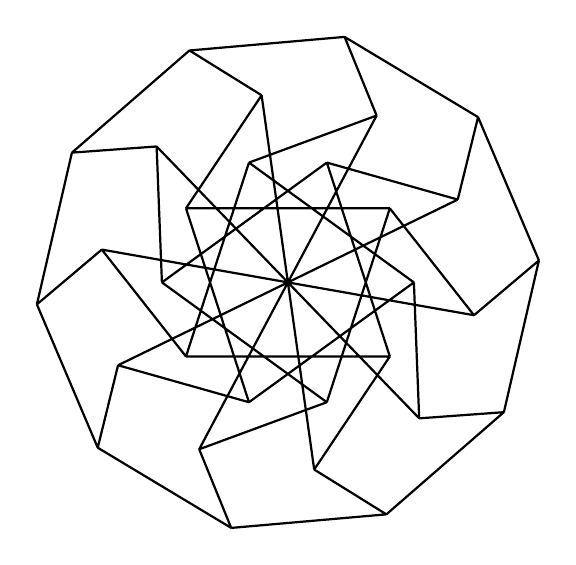
\begin{tikzpicture}[thick,scale=0.8]
    \draw \foreach \x in {0,36,...,324}
    {
        (\x:2) node {}  -- (\x+108:2)
        (\x-10:3) node {} -- (\x+5:4)
        (\x-10:3) -- (\x+36:2)
        (\x-10:3) --(\x+170:3)
        (\x+5:4) node {} -- (\x+41:4)
    };
\end{tikzpicture}\quad
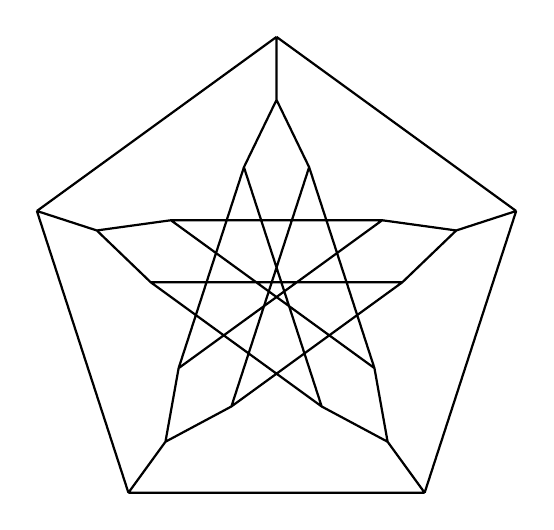
\begin{tikzpicture}[thick,scale=0.8]
    \draw \foreach \x in {18,90,...,306} {
        (\x:4) node{} -- (\x+72:4)
        (\x:4) -- (\x:3) node{}
        (\x:3) -- (\x+15:2) node{}
        (\x:3) -- (\x-15:2) node{}
        (\x+15:2) -- (\x+144-15:2)
        (\x-15:2) -- (\x+144+15:2)
};
\end{tikzpicture}
}

\vspace{10pt}
\nid If you are interested in the code that generated those cool graphs, check out the .tex file for this document.  But again, I only have a vague idea about how this code works (so don't ask me questions about it \smiley).  If you are the do-it-yourself type, and into computer programming, then \texttt{tikz} might be your thing.

But one related package that I \textit{have} used is \texttt{tikz-cd}.  This package is an easy-to-use package that is a very simplified version of \texttt{tikz}.  It is streamlined to do one thing very well: it is great for making commutative diagrams (hence the ``cd'' in the name).  Now if you have never heard of a commutative diagram don't worry about it.  But if you are into advanced mathematics these pop up occasionally (in advanced algebra, topology, manifold theory etc.).  They are essentially diagrams that map out the relationships between functions.  Here is an example that you might see in a smooth manifolds course.  Suppose you have the following  four functions defined on the following sets: 
\begin{align*}
q&:U\rightarrow\widetilde{U}\\
\varphi&: U\rightarrow \mathbb{B}^n\\
\widetilde{\varphi}&:\widetilde{U}\rightarrow \mathbb{R}^n\\
\widehat{q}&: \mathbb{B}^n \rightarrow \mathbb{R}^n.
\end{align*}
\nid Furthermore, suppose these functions commute, meaning: $\widetilde{\varphi}\circ q = \widehat{q}\circ \varphi$.  Then it is very nice to depict the relationship between these functions with a commutative diagram like this: 
\begin{center}
\begin{tikzcd}
U \arrow{r}{q} \arrow{d}[swap]{\varphi}
& \widetilde{U} \arrow{d}{\widetilde{\varphi}} \\
\mathbb{B}^n \arrow{r}{\widehat{q}}
& \mathbb{R}^n
\end{tikzcd}
\end{center}
The arrows show the direction of the mappings and the overall picture is much clearer.

Here is the code that created that in case you are interested (think of the code as two lines in an align environment but with connected arrows):
\begin{verbatim}
\begin{center}
\begin{tikzcd}
U \arrow{r}{q} \arrow{d}[swap]{\varphi}
& \widetilde{U} \arrow{d}{\widetilde{\varphi}} \\
\mathbb{B}^n \arrow{r}{\widehat{q}}
& \mathbb{R}^n
\end{tikzcd}
\end{center}
\end{verbatim}
If you want information about this package see:
\begin{center}
\url{http://www.ctan.org/pkg/tikz-cd}
\end{center}
\subsection{Adding figures with \texttt{graphicx}}
Now it is time to learn the more common, every-day method for adding figures to your document.  I will keep things simple here with some easy to copy examples.  My intent is to explain the topic to someone who is new to this.  If you want to jump right to a more detailed presentation on adding graphics, by all means go here:\\

\url{http://en.wikibooks.org/wiki/LaTeX/Importing_Graphics}\\

\nid But my presentation here will hopefully be sufficient for most basic purposes.  

We will need two new packages in this section which I have never mentioned before: \texttt{graphicx} and \texttt{caption}.  The \texttt{graphicx} package will help us handle adding the figures and the \texttt{caption} package makes adding captions to your figures very easy.

When you add figures to your document with \texttt{graphicx}, you will be adding a preexisting picture file to your document.  This picture file needs to be saved in same working directory as the .tex file that you are compiling.\footnote{Well... that is not the whole story but I am trying to keep it simple.  You can actually add pictures from anywhere on your computer using the \texttt{\textbackslash graphicspath} command.  See the section entitled ``Graphics storage'' here for more on this:\\\url{http://en.wikibooks.org/wiki/LaTeX/Importing_Graphics}}

When you are adding graphics to your \LaTeX\ document with \texttt{graphicx}, make sure you are compiling your document with the pdf\LaTeX\ option.  Your \LaTeX\ editor should have an option controlling what format it will create after it compiles your document.  In \TeX works, for example, there is a pull down menu next to the compile button.  I use \TeX studio and pdflatex is the default choice.  If you build your file with the pdflatex option, then you can add any of the following picture file types to your document:
\begin{multicols}{2}
\begin{itemize}
\renewcommand{\labelitemi}{$\triangleright$}
\item \texttt{.jpg}
\item \texttt{.png}
\item \texttt{.pdf}
\item \texttt{.eps}
\end{itemize}
\end{multicols}

An \texttt{.eps} file format is similar to a \texttt{.pdf} and stands for Encapsulated Postscript (you will likely see references to this in \LaTeX\ documentation).  The two file formats on the left are for bitmaps and the two on the right are for vector graphics.\footnote{I mentioned earlier that I like to use Inkscape to create vector graphic drawings.  By default, Inkscape saves in the \texttt{.svg} format, but it has a option of saving as a \texttt{.pdf}.  So when I do a drawing in Inkscape, I save it as a \texttt{.pdf} and then use \texttt{graphicx} to add that file to my \LaTeX\ document.}

\subsubsection{Adding pictures in a fixed position}\label{sec:fixedpositionpics}
To add a picture to your document all you just need to have the \texttt{graphicx} package added in your preamble and then you can use\\

\nid\verb|\includegraphics[options]{filename}|\\

\nid In all of the examples in this section, this function will add a picture in precisely in the place where you put this command.   The \texttt{filename} is the name of the picture file that you want the \texttt{graphicx} package to pull into your document.   (In section \ref{sec:captionsandfloats} we will cover how to add pictures is such a way that you will let \LaTeX\ decide the best place to fit the picture.) I will explain the \texttt{options} in a minute; you are not required  to specify any options.  For the \texttt{filename}, I recommend you only type the name of the picture file and do not add the extension (like .jpg or .pdf etc.).  Just make sure that all of your picture files that you are adding to your document are in your working directory and have different file names.  In my current directory I have a file called \texttt{alice.jpg} which is a bitmap file of one of the original illustrations of Alice from \textit{Alice in Wonderland} (illustration by John Tenniel in 1865). To add this picture to my document all I need is this:\\

\verb|\includegraphics{alice}|\\

\nid If I didn't have a file in my current directory with the name ``alice,'' I would get an error.  The result of this code is so large that it will end up filling almost all of the next page.\\

\vfill
\pagebreak

\includegraphics{alice}

\nid Since I didn't provide any optional arguments to the \verb|\includegraphics| function, the picture was blown up to fill the page.  If you want to make the image smaller you can add the optional input \verb|scale=| inside square brackets.  You then set the scale option equal to a scale multiplier.  So let's make Alice shrink (don't worry, Alice is quite accustomed to shrinking... she is about to drink the vial of liquid you know):\\

\verb|\includegraphics[scale=0.25]{alice}|\\

\nid I will put the result of this code on it's own line:\\

\includegraphics[scale=0.25]{alice}

\nid This shrunk Alice to a quarter of her original size.  You might notice that the picture is indented, that is because I put the picture on it's own line after a \verb|\\| and \LaTeX\ treats this picture just like adding a symbol or text.  

You can also specify the options \verb|width| and/or \verb|height| in a similar way to \verb|scale|.  You just set them equal to whatever length you want with whatever units you want. If you only specify either \texttt{height} or \texttt{width} (but not both), then the proportions (aspect ratio) of the image will be preserved.  But if you specify both lengths the image will be stretched to exactly those dimensions.  Here is an example of all three.  The third example has two optional arguments so you need a comma separating the multiple arguments:

\begin{verbatim}
\noindent
\includegraphics[height=2in]{alice}
\includegraphics[width =2in]{alice}
\includegraphics[height=4in, width=3in]{alice}
\end{verbatim}
\noindent
\includegraphics[height=2in]{alice}
\includegraphics[width =2in]{alice}
\includegraphics[height=4cm, width=3in]{alice}

\nid The first one is 2 inches tall and the width adjusts proportionally. Similarly, the second picture is 2 inches wide and the height adjusts proportionally.  But the third picture is forced to the specified dimensions and thus is distorted. Also, the forced dimension caused it to overflow into the margin (so you have to pay attention to your output).  Also notice that in the last code example above, I added the three figures in succession without any newline command.  These three figures are added on the same line just as if I typed three letters or math symbols in succession.  Adding a picture is just like adding any symbol; it just takes up more space.  Since the pictures act just like text, I used \verb|\noindent| at the beginning of the line since I wanted the pictures to be flush with the left margin.  The bottom of the figures are on the same line.  So if you have text in the same line as a picture it will be in the same line like this:

\begin{verbatim}
\includegraphics[scale=0.1,angle=90]{alice}
$\Leftarrow$ Alice rotated $\Rightarrow$ 
\includegraphics[angle = -30, scale=0.15]{alice} 
\end{verbatim}

\includegraphics[scale=0.1,angle=90]{alice}
$\Leftarrow$ Alice rotated $\Rightarrow$ 
\includegraphics[angle = -30, scale=0.15]{alice}

\nid The example above also shows how you can rotate a picture as well.  Positive angles rotate counterclockwise and the units are in degrees.

Now, all of the figures I have added in the examples above have been added inline, but you can also add figures inside of an environment like \verb|center|.  In the next example I will also show you how you can set the width to be a multiple of the width of the page so you don't have to choose a specific width.  
\begin{verbatim}
\begin{center}
\includegraphics[width=.45\columnwidth]{alice}
\end{center}
\end{verbatim}
\nid This will make the picture centered and it will fill up 35\% of the width of the main text column.  Instead of \verb|\columnwidth| you can substitute \verb|\linewidth| or \verb|\textwidth| if you like.  I like to use \verb|\columnwidth| because it works inside of a multicolumn environment to fit the thinner column.  Here is the result of the last code example:\phantomsection\label{blankspace}
\begin{center}
\includegraphics[width=.45\columnwidth]{alice}
\end{center}

If you want to crop a picture you can do that too.  You need to add the argument \verb|clip=true| to  the optional arguments and then \verb|trim=| followed by four lengths representing how much you are going to trim from the \textsl{left}, \textsl{bottom}, \textsl{right} and \textsl{top} in that order.  The following code is an example of a cropped picture inside the \texttt{flushright} environment.  I will trim 2cm of the left 12cm off the bottom, 3cm off the right and 0cm off the top.  Then the result will be rescaled to fit 30\% of the column width (it is not exactly obvious how the trimming will look; you sort-of have to play around with crop lengths and keep building the file and see what happens):\\

\begin{verbatim}
\begin{flushright}
\includegraphics[width=.3\columnwidth,trim=2cm 12cm 3cm 0cm,clip=true]{alice}
\end{flushright}
\end{verbatim}
\nid Here is the result:

\begin{flushright}
\includegraphics[width=.3\columnwidth, trim=2cm 12cm 3cm 0cm, clip=true]{alice}
\end{flushright}

You can also reflect a picture by putting it inside a \verb|\reflectbox{}| which flips anything inside of it right to left (let me emphasize that you can flip anything, including text, in a \verb|\reflectbox{}|):
\begin{verbatim}
\begin{center}
\reflectbox{\includegraphics[width=3.5in]{alice}}
\end{center}
\end{verbatim}


\begin{flushright} \reflectbox{So here is Alice after she has gone through the looking glass:}
\end{flushright} 

\begin{center}
\reflectbox{\includegraphics[width=2in]{alice}}
\end{center}

\subsubsection{Captions and floats}\label{sec:captionsandfloats}
A ``float'' is a certain special type of object in \LaTeX.  Floats are given the name ``float'' because they will not necessarily be created exactly where you put them in your code.  Instead, when you create a float, you allow \LaTeX\ to decide \textit{where} it will best be placed in the document so that it looks good.  The two main types of floats that are available in \LaTeX\ are \textsl{figures} and \textsl{tables}.  To create a figure or a table you need to use the \texttt{figure} or \texttt{table} environment.  Up to this point I have not taught you how to create a figure or a table, so I have never explicitly taught you how to make a floating object yet.  In this section I will explain how to make a floating figure with the \texttt{figure} environment (I will explain tables in a later section).  But first I want to emphasize that none of the pictures that we added in the previous two sections were added in the \texttt{figure} environment so \textit{none} of them were floats.  All of the pictures we added above were added to the document exactly where we declared them, either right in-line, or inside of an environment like \texttt{center} or \texttt{flushright} (which are not floating environments).  But you \textit{can} include a picture inside of a \texttt{figure} environment and then the picture will become a float. The downside to adding pictures in the way we did above, is that you might get a bunch of awkward empty space in some places. See for example, the bottom of page \pageref{blankspace}, where we added a picture of Alice that filled up 45\% of the columnwidth.  That picture was too big to fit the rest of the page in that situation, so it forced the picture to the top of the following page, which left a lot of unused blank space at the bottom of page \pageref{blankspace}.  When you use the \texttt{figure} environment, this will not happen.  \LaTeX\ will move the figure around and adjust the text so that there won't be blank space. It's time for an example.

The following is an example using the figure environment.  I will show you the code here and then I will explain it below.  This example also shows you how to give a figure a caption using the \verb|caption| package and I also label the figure so we can reference it later:
\begin{verbatim}
\begin{figure}
\centering
\includegraphics[width=0.6\columnwidth]{teaparty}
\caption[A Mad Tea-Party]{From left to right we see Alice, the March Hare, the 
Doormouse, and the Hatter.}
\label{fig:teaparty}
\end{figure}
\end{verbatim}
\begin{figure}
\centering
\includegraphics[width=0.6\columnwidth]{teaparty}
\caption[A Mad Tea-Party]{From left to right we see Alice, the March Hare, the Doormouse, and the Hatter.}
\label{fig:teaparty}
\end{figure}
Even though I added this code example \textit{before} I typed this paragraph, \LaTeX\ floated the picture to the top of the next page because it fits better there.  So it isn't leaving any empty space on this page.  You should look at the code in the .tex file to see what I mean.  In the example code above, I am adding the picture file \texttt{teaparty.jpg} inside of the figure environment in the exact same way I explained in the sections above.  The only thing that is new is that it is inside of the figure environment.  I used the \verb|\centering| function to center what is inside of the figure environment.  This is not quite the same as using the \texttt{center} environment.  I recommend you only use the \verb|\centering| command inside of another environment like I am doing here (or inside of any box that creates a paragraph).\footnote{For more on the differences between the \texttt{center} environment and the \texttt{centering} command, see:\\
\url{http://tex.stackexchange.com/questions/23650/when-should-we-use-begincenter-instead-of-centering}} When you create a figure you can easily add a caption with the \texttt{caption} package which gives you the function \verb|\caption[list entry]{caption text}|.  The first, optional argument to this function is in square brackets.  This \verb|list entry| is the text that gets added to the list of figures that you see on page \pageref{listoffigures}.  The second argument in curly braces is the caption that is added below the actual figure.  Make sure to put the \verb|\caption| function right after the \verb|\includegraphics| line.  When you add a caption, it creates a figure number which you can label and reference with the same methods we learned in part 1 of the introduction to \LaTeX.  Only figures that have numbers will be added to the list of figures that you see on page \pageref{listoffigures}.  If you want a caption but you don't want the figure to be numbered, you can use the \verb|caption*{caption text}| version of the function instead.

Because we labeled the Mad Tea-Party picture, we can reference it.  If we type:\\

\nid\verb|In figure \ref{fig:teaparty} we see John Tenniel's Mad Tea-Party illustration.|\\

\nid This, of course, is the result:\\

\nid In figure \ref{fig:teaparty} we see John Tenniel's Mad Tea-Party illustration.\\

By-the-way, I mentioned the list of figures at the beginning of the document.  That is very easy to create.  All you have to do is type \verb|\listoffigures| wherever you want it to go, and it will automatically be formatted for you.  It works just like \verb|\tableofcontents|.

Now sometimes you might not like the place where \LaTeX\ places your float.  If that ever happens you have some options.  One is to add one (or more) of the various optional placement commands to the \texttt{figure} environment declaration.  These go in square brackets like the one you can see here (I have added the \texttt{t!} commands):
\pagebreak

\begin{verbatim}
\begin{figure}[t!]
\centering
\includegraphics[width=0.3\columnwidth]{alice}
\caption{Alice}{Drink me!}
\label{fig:drinkme}
\end{figure}
\end{verbatim}
\begin{figure}[t!]
\centering
\includegraphics[width=0.5\columnwidth]{alice}
\caption[Alice]{Drink me!}
\label{fig:drinkme}
\end{figure}
If you just put a \texttt{t} in the square brackets, then you are requesting that \LaTeX\ to \textit{try} to put the float at the top of the page.  By adding the \texttt{!} I am \textit{asking} \LaTeX\ to break the rules and do anything it can to try and force the picture to be at the top of the page (but even this doesn't always work though). If you want to learn more optional placement commands that are available, read this page which has a lot of details:\\

\nid\url{http://en.wikibooks.org/wiki/LaTeX/Floats,_Figures_and_Captions}\\

There are some drawbacks to using floating figures.  If your document has a lot of figures that are very close together with very little text in between, then \LaTeX\ will have difficulty figuring out where to put everything.  So if I would have done section \ref{sec:fixedpositionpics} with all floats instead of forcing the pictures, it would not have worked.  Also there might be times where you want a sequence of figures one right after the other and you don't want any text between them (like if you are showing still frames of something that is changing over time).  This generally will not work well with floating figures. If you want a bunch of picture in a row, especially if you want them to take up a complete page or more, it is best to use fixed position pictures like we had in section \ref{sec:fixedpositionpics}.

So forcing the position of a picture can be the best way to go, but \LaTeX\ on it's own will not number any fixed position picture using the methods in section \ref{sec:fixedpositionpics}.  But fortunately the \texttt{caption} package has a solution for this with the alternate function \verb|\captionof|. So if you want to create a figure with a caption but you want to force the positioning this this the method: first, you have to add the figure inside of some \emph{non-floating} environment like \verb|center| or \verb|flushleft|.  Second, after you include the graphic, you use the function:\\
\verb|\captionof{float type}[list entry]{caption text}|.\\
Again, the \verb|list entry| is the text that goes in the list of figures and the \verb|caption text| is what goes directly below the figure.  The \verb|float type| is needed becaues this caption is not inside of the \texttt{figure} environment but \LaTeX\ needs to know which list to put this figure on.  So even though this example isn't inside of an actual float, you need to specify the ``float type'' so that \LaTeX\ knows how to number the caption.  The float type should either be ``figure'' or ``table'' (unless you use some other custom float type which I won't explain here).  Figure \ref{fig:circle} below is a mathematical figure that uses this method of forcing a fixed position but with a figure caption.  In the example I choose the float type to be \verb|figure| so that the number that is given puts it in the list of figures in the correct order.  This is a picture that I drew in Inkscape to demonstrate the concept of projecting a circle from a sphere to a plane via stereographic projection.  Here is the code:\\

\begin{verbatim}
\begin{center}
\includegraphics[width=.75\columnwidth]{RiemannSphereCircle}
\captionof{figure}[A circle on the Riemann sphere.]{The Riemann sphere 
$\mathbb{S}^2$ is shown.  The red rays, etc.}
\label{fig:circle}
\end{center}
\end{verbatim}
\begin{center}
\includegraphics[width=.75\columnwidth]{RiemannSphereCircle}
\captionof{figure}[A circle on the Riemann sphere.]{The Riemann sphere 
$\mathbb{S}^2$ is shown.  The red rays, which emanate from the north pole $(0,0,1)$, show the process of stereographic projection of points on the sphere to points in the complex plane $\mathbb{C}$.  The intersection of a plane with the sphere is a circle \emph{on the sphere} and the projection of this intersection is a standard Euclidean circle \emph{in the plane}.}
\label{fig:circle}
\end{center}

So this shows you that your figure caption can have math and various script styles as well.  Because I created this picture in Inkscape, it is a vector graphics file.  I saved the file as a .pdf in Inkscape, which allowed me to easily add it to this document with the \texttt{graphicx} package.  You should view this document in Adobe reader and zoom in on figure \ref{fig:circle}.  You will find that the lines stay sharp.  Then zoom in on the bitmap picture in figure \ref{fig:teaparty} and you will see that the picture degrades as you zoom in.

The last thing I will show you how to do in this section is to add subfigures inside of a figure.  But I need to warn you that the methods I use here \textit{might} clash with other packages that you will want to use.  Everything I do here works just fine with the packages that I have chosen for this document though (and most likely these methods will work for you in general).  This method uses the \verb|subfigure| environment but some people recommend using the package called \verb|subfig| instead (which I am not using here).\footnote{There are conflicting opinions about what is correct here.  I think if you use the \texttt{subcaption} package you will be just fine.  If this is important to you, then you can find out more about these issues at the following sites:\\
\url{http://en.wikibooks.org/wiki/LaTeX/Floats,_Figures_and_Captions}\\
\url{http://www.ctan.org/pkg/subcaption}\\
\url{http://www.ctan.org/pkg/subfig}\\
\url{http://tex.stackexchange.com/questions/144782/subfigure-and-subfig-packages-deprecated}}
O.k., with all of the mild warnings aside here is how it works.  You need to add the \verb|subcaption| package to your preamble (which I have done).  This package provides you with a new environment \verb|\begin{subfigure}[optional position]{mandatory width}|.  This environment allows you to add subfigures inside of a figure.  The ``optional position'' in brackets is not necessary when you use it in the way that I will use it here , and I have never needed it anywhere.  But you might someday, so read the documentation on \texttt{subcaption}.  (See the footnote with the link.)  The ``mandatory width'' is the width of the box that holds the subfigure.   To see an example, the result of the following code example can be seen in figure \ref{fig:threepics}.  The cool thing about subfigures is that you can give a caption to the subfigures inside of the figure and \emph{also} give a caption to the whole figure.  The subfigure captions will create a sub-lettering that will allow you to label and reference the subfigures as well.  This is extremely useful when you are comparing multiple figures side-by-side in a mathematical paper.  Here is the code for the example and I will explain some of the details below the code block:
\begin{verbatim}
\begin{figure}[b]
\centering
\begin{subfigure}{0.2\textwidth}
\includegraphics[width=\textwidth]{alice}
\caption{Alice}
\label{subfig:alice}
\end{subfigure}
\quad
\begin{subfigure}{0.35\textwidth}
\includegraphics[width=\textwidth]{teaparty}
\caption{Mad Tea-Party}
\label{subfig:teaparty}
\end{subfigure}
\quad
\begin{subfigure}{0.35\textwidth}
\includegraphics[width=\textwidth]{RiemannSphereCircle}
\caption{The Riemann Sphere}
\label{subfig:sphere}
\end{subfigure}
\caption[A figure with subfigures]{This example shows how to have subfigures 
inside of a figure, create captions for all of them, label them, and later 
reference them separately. Notice that the code for this caption also creates the 
text that you see in the list of figures at the beginning of the document.}
\label{fig:threepics}
\end{figure}
\end{verbatim}
\begin{figure}[b]
\centering
\begin{subfigure}{0.2\textwidth}
\includegraphics[width=\textwidth]{alice}
\caption{Alice}
\label{subfig:alice}
\end{subfigure}
\quad
\begin{subfigure}{0.35\textwidth}
\includegraphics[width=\textwidth]{teaparty}
\caption{Mad Tea-Party}
\label{subfig:teaparty}
\end{subfigure}
\quad
\begin{subfigure}{0.35\textwidth}
\includegraphics[width=\textwidth]{RiemannSphereCircle}
\caption{The Riemann Sphere}
\label{subfig:sphere}
\end{subfigure}
\caption[A figure with subfigures]{This example shows how to have subfigures inside of a figure, create captions for all of them, label them, and later reference them separately. Notice that the code for this caption also creates the \texttt{list entry} text that you see in the list of figures at the beginning of the document.}
\label{fig:threepics}
\end{figure}
Notice that I added the optional \verb|[b]| to the \texttt{figure} environment declaration.  This is a request to \LaTeX\ to put the figure at the bottom of the page. I actually don't think it is a good idea in this case to force the bottom position;  I would prabably not have the optional positioning at all.  I just threw it in to show you that you \emph{can do this} if you want, and I wanted to show you the results.  Also note that each of the three pictures in this example are added \textit{inside} of their own \texttt{subfigure} environment and all of these are nested inside of the \texttt{figure} environment.  So the entire block of pictures is one floating figure object, but the three pictures will be side-by-side in the same line (once \LaTeX\ decides it's final position).  To put a bit of space between the figures I put a \verb|\quad| space between each picture.  Also note that the width of the first subfigure is 20\% of the \verb|\textwidth| and the second two take up 35\%.  I did this so that the proportions look good next to each other since the first picture is taller than it is wide.  But also note that I made the width of the pictures equal to the \verb|\textwidth|.  This will ensure that the picture fills up the entire width of the subfigure box.  It is important where I placed the captions and labels as well.  The caption for the subfigures come right after the lines that include the picture file, and the caption for the entire figure comes right after the last subfigure environment is ended.  Then the labels for each of the four captions come right after the corresponding caption.  This order is important because you need to make sure you are tying the label to the caption which is creating the numbering for the label, and you want to make sure the caption is placed under the right picture.  You will get errors if you change the order.  And sometimes I have found that if you have blank lines of code in the environment it will cause problems so avoid having blank lines in your code. 

Now that we have created this cool figure and labeled everything we can reference these labels in a variety of ways using \verb|\ref|, \verb|\eqref| (which we covered in part 1 of the introduction) and the new option we have never seen before: \verb|\subref|.  We get \verb|\subref| from the \verb|subcaption| package.  Here is an example that combines all the different ways you might want to format your references to the figure and subfigures (take note of where I manually added parentheses and where I didn't):
\begin{verbatim}
Figure \ref{fig:threepics} shows a figure with subfigures.  Figure 
\ref{subfig:alice} and \eqref{subfig:teaparty} are bitmaps but figure 
\ref{fig:threepics}(\subref{subfig:sphere}) is a vector drawing.  It seems that 
\subref{subfig:alice} and \subref{subfig:teaparty} in figure \eqref{fig:threepics} 
go together but figure (\subref{subfig:sphere}) doesn't fit in.
\end{verbatim}
\nid Here is the result of this code:\\

Figure \ref{fig:threepics} shows a figure with subfigures.  Figure \ref{subfig:alice} and \eqref{subfig:teaparty} are bitmaps but figure \ref{fig:threepics}(\subref{subfig:sphere}) is a vector drawing.  It seems that \subref{subfig:alice} and \subref{subfig:teaparty} in figure \eqref{fig:threepics} go together but figure (\subref{subfig:sphere}) doesn't fit in.


% % % % % % % % % % %NEW SECTION % % % % % %
%
%
%		BibTeX
%
%
% % % % % % % % % % % % % % % % % %5 % % % %
\section{How to make a bibliography with BiB\TeX}\label{sec:bibtex}
Another really awesome thing that \LaTeX\ can do for you is create a bibliography for you with a minimal amount of work on your part.  You won't have to spend hours fiddling with commas, periods, abbreviations, etc.  You won't even have to worry much about the differences between MLA, APA, or Chicago styles (or the many different styles available).  You will simply enter in all of the information about your citation into a list of information, then tell \LaTeX\ what style you want, and it will format it all for you.  In fact you can do even better than that! If you use Google Books or Google Scholar correctly then you can download all of this info in the correct format instantly, copy paste it to your file and you are done! 

So, in this section I will show you the basics on how to make a bibliography and how the code needs to be organized, but I won't go over all of the many possible types of citations you might have.  Once you know the coding part, I will direct you to online resources that have the details and examples you need.

I should at least mention the various methods for making bibliographies that I \emph{am not} going to explain, just so you know they exist.  Then you could go learn them on your own if you want to.  It turns out that there are a few different bibliography methods that each have their strengths and weaknesses.  One option is to make the citations yourself using the environment called \texttt{thebibliography} and the function \verb|\bibitem{}|.  This is a direct do-it-yourself approach that is fine if you just have one or two citations.  If you want to know more about this see this site:\\

\nid\url{http://www.math.uiuc.edu/~hildebr/tex/bibliographies.html}\\

\nid or read the section 1 of this wikibook entry:\\

\nid\url{http://en.wikibooks.org/wiki/LaTeX/Bibliography_Management}\\

\nid Another option is to use the package called \texttt{natbib} which used to be popular and many people still use it, but it is no longer supported.  I have read that many journals require \texttt{natbib} if you want to get a paper published.  If you wish to know more about this see section 2.4 here:

\nid\url{http://en.wikibooks.org/wiki/LaTeX/Bibliography_Management}\\

\nid or read the documentation here:\\
\nid\url{http://www.ctan.org/pkg/natbib}\\

The bibliography method that I will explain here uses BiB\TeX, which you can think of as a supplement to \LaTeX\ that came bundled with your distribution.  You don't need to add any packages to get it to work.  It runs on the side of \LaTeX.  BiB\TeX, is widely used and has become quite popular.  You should know that there is a newer updated replacement of BiB\TeX, called BiB\LaTeX,  which may eventually completely replace BiB\TeX.  I don't know much about it but here is the documentation:\\

\nid \url{http://www.ctan.org/pkg/biblatex}\\

\nid And there is even one more option that I had never heard of until recently called \texttt{biber}.  You can find a great discussion comparing the benefits and drawbacks of all four of these different bibliography management systems here:\\

\nid\url{http://tex.stackexchange.com/questions/25701/bibtex-vs-biber-and-biblatex-vs-natbib}\\

But since BiB\TeX\ is one of the most widely used, I will focus in it only.  Once you know how it works you could learn the others easily.

When you use BiB\TeX, all of your citation information is stored in a separate file that you need to save with the extension \verb|.bib| instead of \verb|.tex|.  Once you create this \verb|.bib| file, you have to save it in the same directory as your \verb|.tex| file. You can give your \verb|.bib| file any name you want.  For this demonstration lets call our \verb|.bib| file \myrefs.  If you want to compile this document, you will have to download the \verb|.bib| file that goes with this document.

A \verb|.bib| file is fairly simple.  You do not need a preamble of any kind and there are no environments or anything like that.  A \verb|.bib| file is just a formatted data base of information. That is it.  Here is an example of an entry that I added to \myrefs.  This is a typical book citation.  This happens to be a book that I have at my desk as I am typing this.  Here is what I added to the \myrefs\ file:
\begin{verbatim}
@book{LeeTopMan,
  title={Introduction to Topological Manifolds},
  author={John M. Lee},
  series={Graduate Texts in Mathematics},
  year={2010},
  publisher={Springer}
}
\end{verbatim}

\nid The beginning of a citation always begins with the \verb|@| character followed by the type of citation.  This is a book so that is what I put (there are many options other than book, which I explain below). Then this is followed by a open curly brace, which is followed by the citation key.  I chose to make the key \verb|LeeTopMan|.  The key is just the code you will use to cite this source in your text (I will show an example of how to do this below).  The key has no effect on the citation in your bibliography.  The other entries that follow after the key are fairly self-explanatory.  You just need to follow the formatting.  Make sure to use the equal signs as I did above and the commas at the end are important.  Also make sure to have the final closed curly brace at the very end to finish the citation.  If you only wanted this one citation in your bibliography, then what you see above is \emph{all you need} in your entire \verb|.bib| file.  That's it!  Just save it in your working directory and you are done. Then, in your \verb|.tex| file, wherever you want to put your bibliography (usually at the end of your document, right before the \verb|end{document}| line), you need the following two lines of code:
\begin{verbatim}
\bibliographystyle{style}
\bibliography{filename}
\end{verbatim}

In the place of \verb|style|, you need to put the bibliography style that you want to use, and in the place of \verb|filename| you put the name of your \verb|.bib| file that you have saved in your working directory.  Here is what I have at the end of this document:

\begin{verbatim}
\bibliographystyle{plain}
\bibliography{myreferences}
\end{verbatim}

The \verb|plain| style is a common simple bibliography style that comes with \LaTeX, and, of course, \verb|myreferences| is the name of my \verb|.bib| file (note that you \emph{do not} put the file extension, just the name of the file).

So now I can use the key that I made to cite this source anywhere in my document.  So if I quote something from the book, or just want to mention it, I can use the \verb|\cite{keylist}| function.  Here is an example:\\

\nid\verb|A great source for information about topological manifolds is \cite{LeeTopMan}.|\\

\nid This will be the result:

\nid A great source for information about topological manifolds is \cite{LeeTopMan}.

Just to show you one more example, here is another entry that adds a journal article which you will find in \myrefs:
\begin{verbatim}
@article{ghrist2008barcodes,
  title={Barcodes: the persistent topology of data},
  author={Ghrist, Robert},
  journal={Bulletin of the American Mathematical Society},
  volume={45},
  number={1},
  pages={61--75},
  year={2008}
}
\end{verbatim}

Now that we have two entries in our references list, I can show you how to cite two things at once.  Sometimes you want to refer the reader to two sources at the same time like this:\\

\nid \verb|If you are really into topology, you should read \cite{LeeTopMan,ghrist2008barcodes}.|\\

\nid I referenced two citations by typing their both keys separated by a comma.  This is the result:\\

If you are really into topology, you should read \cite{LeeTopMan,ghrist2008barcodes}.\\

I have had an example of a book and an article, but here is a list of other common entry types that you can have in BiB\TeX:
\begin{multicols}{2}
\begin{verbatim}
@article
@book
@booklet
@conference
@inbook
@incollection
@manual
@mastersthesis
@misc
@phdthesis
@proceedings
@techreport
@unpublished
\end{verbatim}
\end{multicols}
\nid Here is a great website that has examples of all of these and it also shows you what it will look like if you choose different bibliography styles as well:\\
\url{https://verbosus.com/bibtex-style-examples.html}\\

In my examples above I only had a few fields like \texttt{author}, \texttt{title}, \texttt{publisher}, etc.  Here is a list of other fields that you can add to your citation:
\begin{multicols}{3}
\begin{verbatim}
address
annote
author
booktitle
chapter
crossref
edition
editor
howpublished
institution
journal
key
month
note
number
organization
pages
publisher
school
series
title
type
volume
year
\end{verbatim}
\end{multicols}

\nid Here is a good website that explains what each one of these are and whether and when you should use them:\\
\url{http://www.fb10.uni-bremen.de/anglistik/langpro/bibliographies/jacobsen-bibtex.html}

There are just a few more things that you need to know about BiB\TeX\ that are essential.  First, you need to know that compiling your references takes a few steps, especially if you are using a more basic \LaTeX editor like \TeX works or \TeX shop.  The first time you compile your document that has references in a \verb|.bib| file, you need to compile the document with the following four steps:
\begin{enumerate}
\item Compile your document using pdf\LaTeX\ in the normal way you would any document.  But it will not completely compile, and it will \emph{seem} like there were errors of some kind.  This is normal.
\item Next you have to run BiB\TeX. This is usually an alternate compile option that is available in your \TeX\ editor.  For example, it is one of the build options in the pull-down menu next to the compile button in \TeX works.  When this step is finished ignore any errors or warning messages you might see.  
\item Next, compile your code in pdf\LaTeX\ again and wait until it finishes, but again, it will show errors and it won't completely compile.  But this is normal.
\item Compile your code in pdf\LaTeX\ one last time and if everything was coded correctly, you are now done.  You should be able to view your document. 
\end{enumerate} 

This sequence is required because BiB\TeX\ runs separately from \LaTeX\ and it has to cross reference across different files.  After you complete this sequence one time, you will be able to make changes to your \verb|.tex| file and compile in the normal way.  You don't have to repeat this sequence every time you make changes.  It is only needed during the first compilation. If you make changes to your \verb|.bib| file you might have to redo this sequence. If you use a more sophisticated \LaTeX\ editor like \TeX studio, then all you have to do is compile once, in the usual way, and \TeX studio will recognize that you are compiling a new \verb|.bib| file and it does the above four-step sequence for you automatically.

By default, the only references that will appear in your table of contents are ones that you explicitly cite in your paper.  If you want to have something in your bibliography that you don't explicitly cite you can use the \verb|\nocite{keylist}| function.  And, of course, in the place of ``\texttt{keylist}'' you type the citation keys you want to appear separated by a comma.  Any citation keys you put in this function will be added to your bibliography.  So any source in your \verb|.bib| file that you do not cite in your paper will not be included.  As an example, I added \verb|\nocite{complexfunctions}| to my code right before the bibliography declaration and this added the book by Jones and Singerman to my bibliography even though it isn't cited explicitly.  If you want \emph{all} entries in your \verb|.bib| file to be in your bibliography, then use an asterisk in the place of your keylist: \verb|\nocite{*}|.  The asterisk causes everything to be added.    The nice thing about this is that you can collect a whole bunch of citations as you do some research and just keep collecting them into on \verb|.bib| file, and then you can decide which ones you will include at the very end.  So you could reuse that same \verb|.bib| file in the future as well (in case you write multiple papers in the same topic area).

Finally, the type of file that contains the code for the bibliography \emph{style} is a \verb|.bst| file.  On my PC with Mik\TeX, these files are saved in the following directory:\\

\verb|C:\Program Files (x86)\MiKTeX 2.9\bibtex\bst|\\

\nid But this may be different on your operating system and \TeX\ distribution. If you can find where the \verb|.bst| files are saved on your computer, then you can find what bibliography styles are available to you.  Here are the different styles that I have on my computer with the standard Mik\TeX\ installation:
\begin{multicols}{3}
\begin{itemize}
\item abbrv
\item acm
\item alpha
\item ieeetr
\item plain
\item siam
\item unsrt
\item amsplain
\item amsalpha
\end{itemize}
\end{multicols}
\nid The last two are variations of the \texttt{plain} and \texttt{alpha} styles that have been created by the American Mathematical Society.  If you want to get more bibliography styles that you don't have, you need to get the \verb|.bst| file for that style.  And you would need to save the file where \LaTeX\ can find it.  So the easiest way is to save the \verb|.bst| file you want to use in your current working directory.  Here is a website from Reed College that has an MLA and APA style if need those:

\url{http://www.reed.edu/cis/help/latex/bibtexstyles.html}

\newpage

\nocite{complexfunctions}
\bibliographystyle{plain}
\bibliography{myreferences}

\end{document}




